\documentclass{beamer}
\usepackage[utf8]{inputenc}
\usepackage[normalem]{ulem}
\usepackage{tikz}
\usepackage{graphicx}

\title{The \sout{Antibac}Buggy}
\author{Kent Odde, Stian Onarheim, Tarald Vestbøstad}
\institute{USN}
\date{Autumn 2020}

\begin{document}

\frame{\titlepage}
\addtobeamertemplate{headline}{}{%
\begin{tikzpicture}[remember picture,overlay]
\node at([shift={(.45\paperwidth,-.64)}]current page.north) {
\includegraphics[height=.5cm]{img/logo.png}};
\end{tikzpicture}}

\begin{frame}
\frametitle{Showcase}
    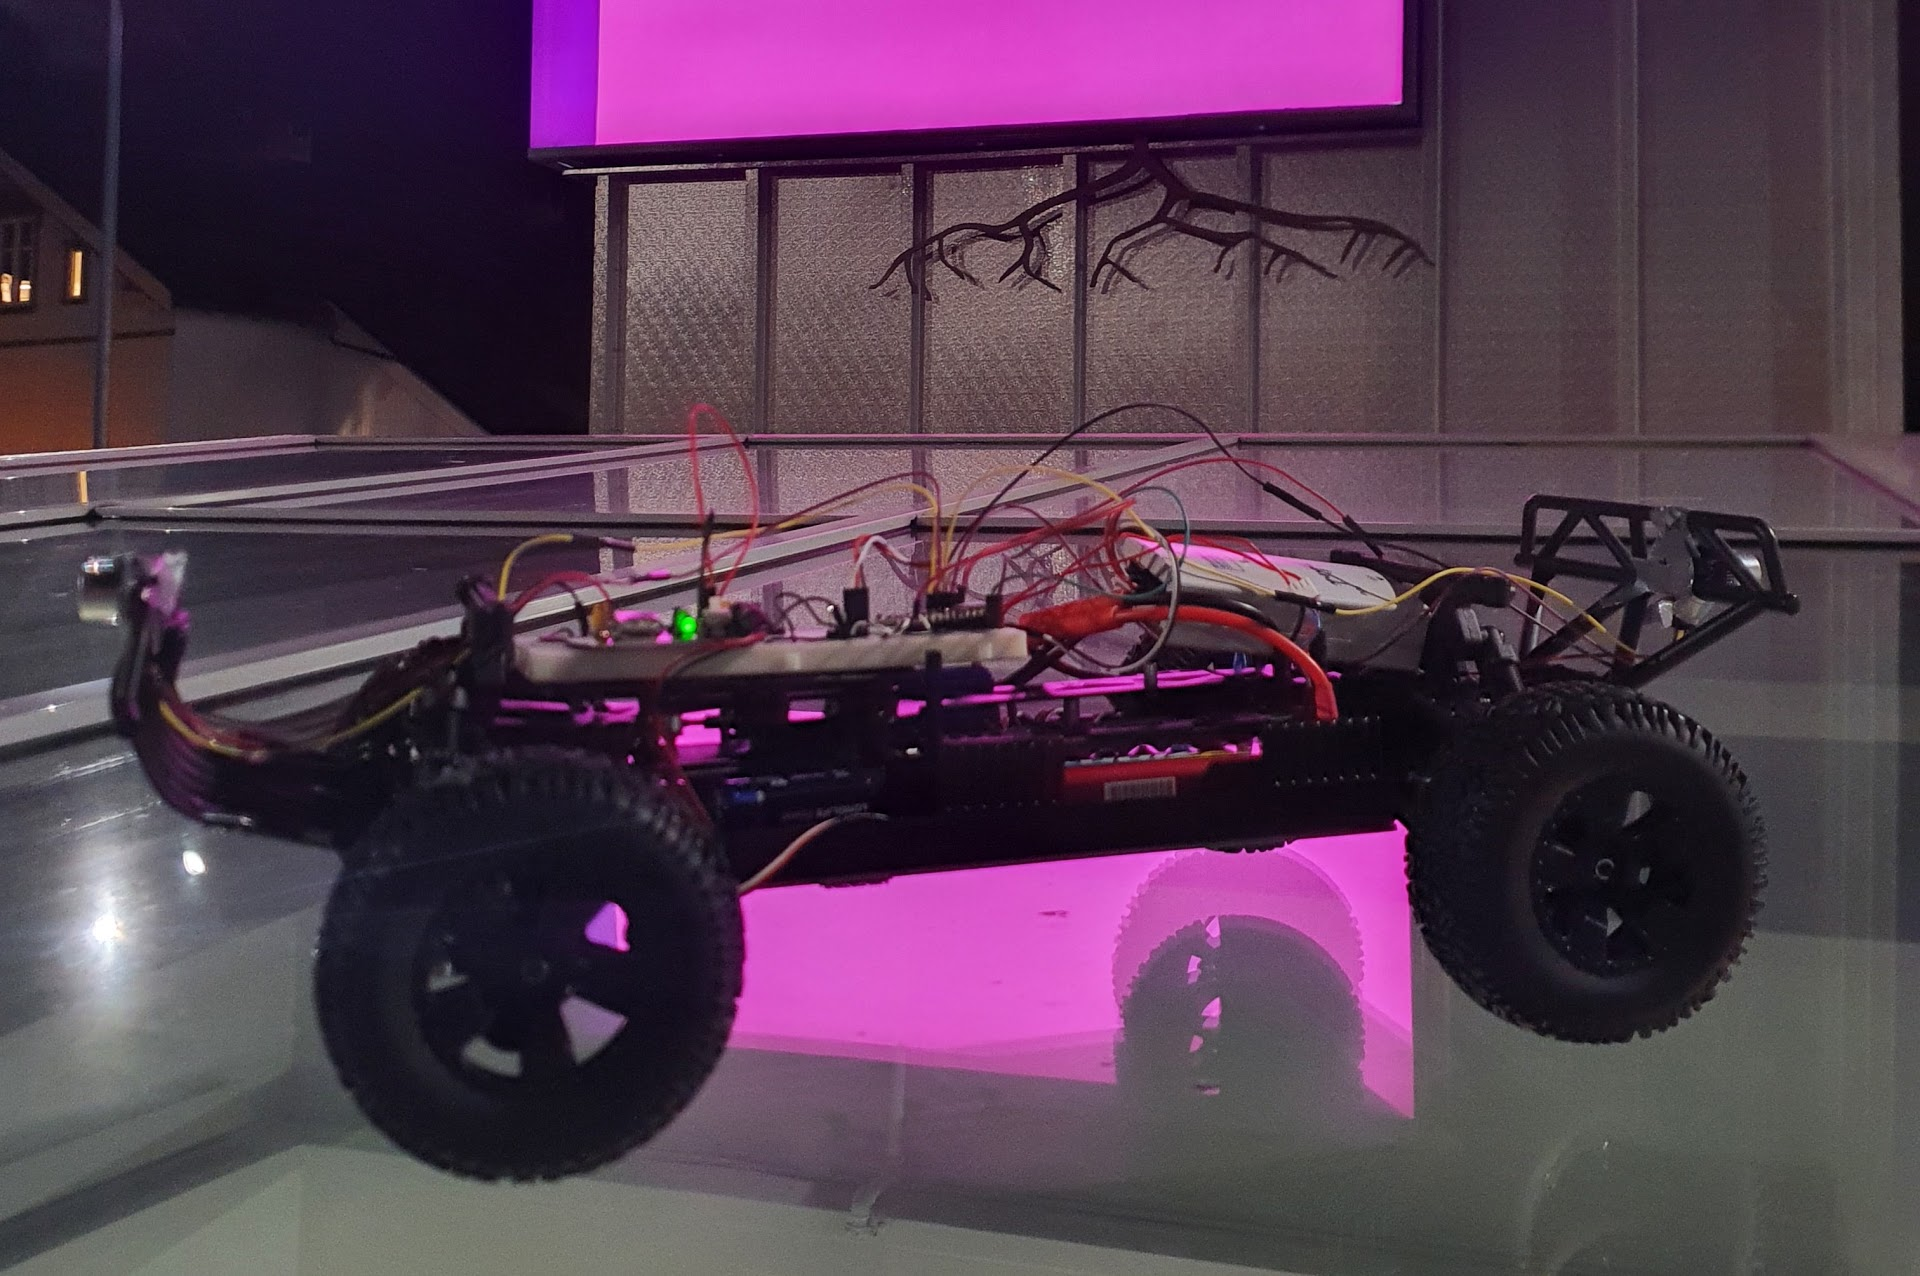
\includegraphics[width=\linewidth]{img/showcase.png}
\end{frame}

\begin{frame}
\frametitle{Timeline}
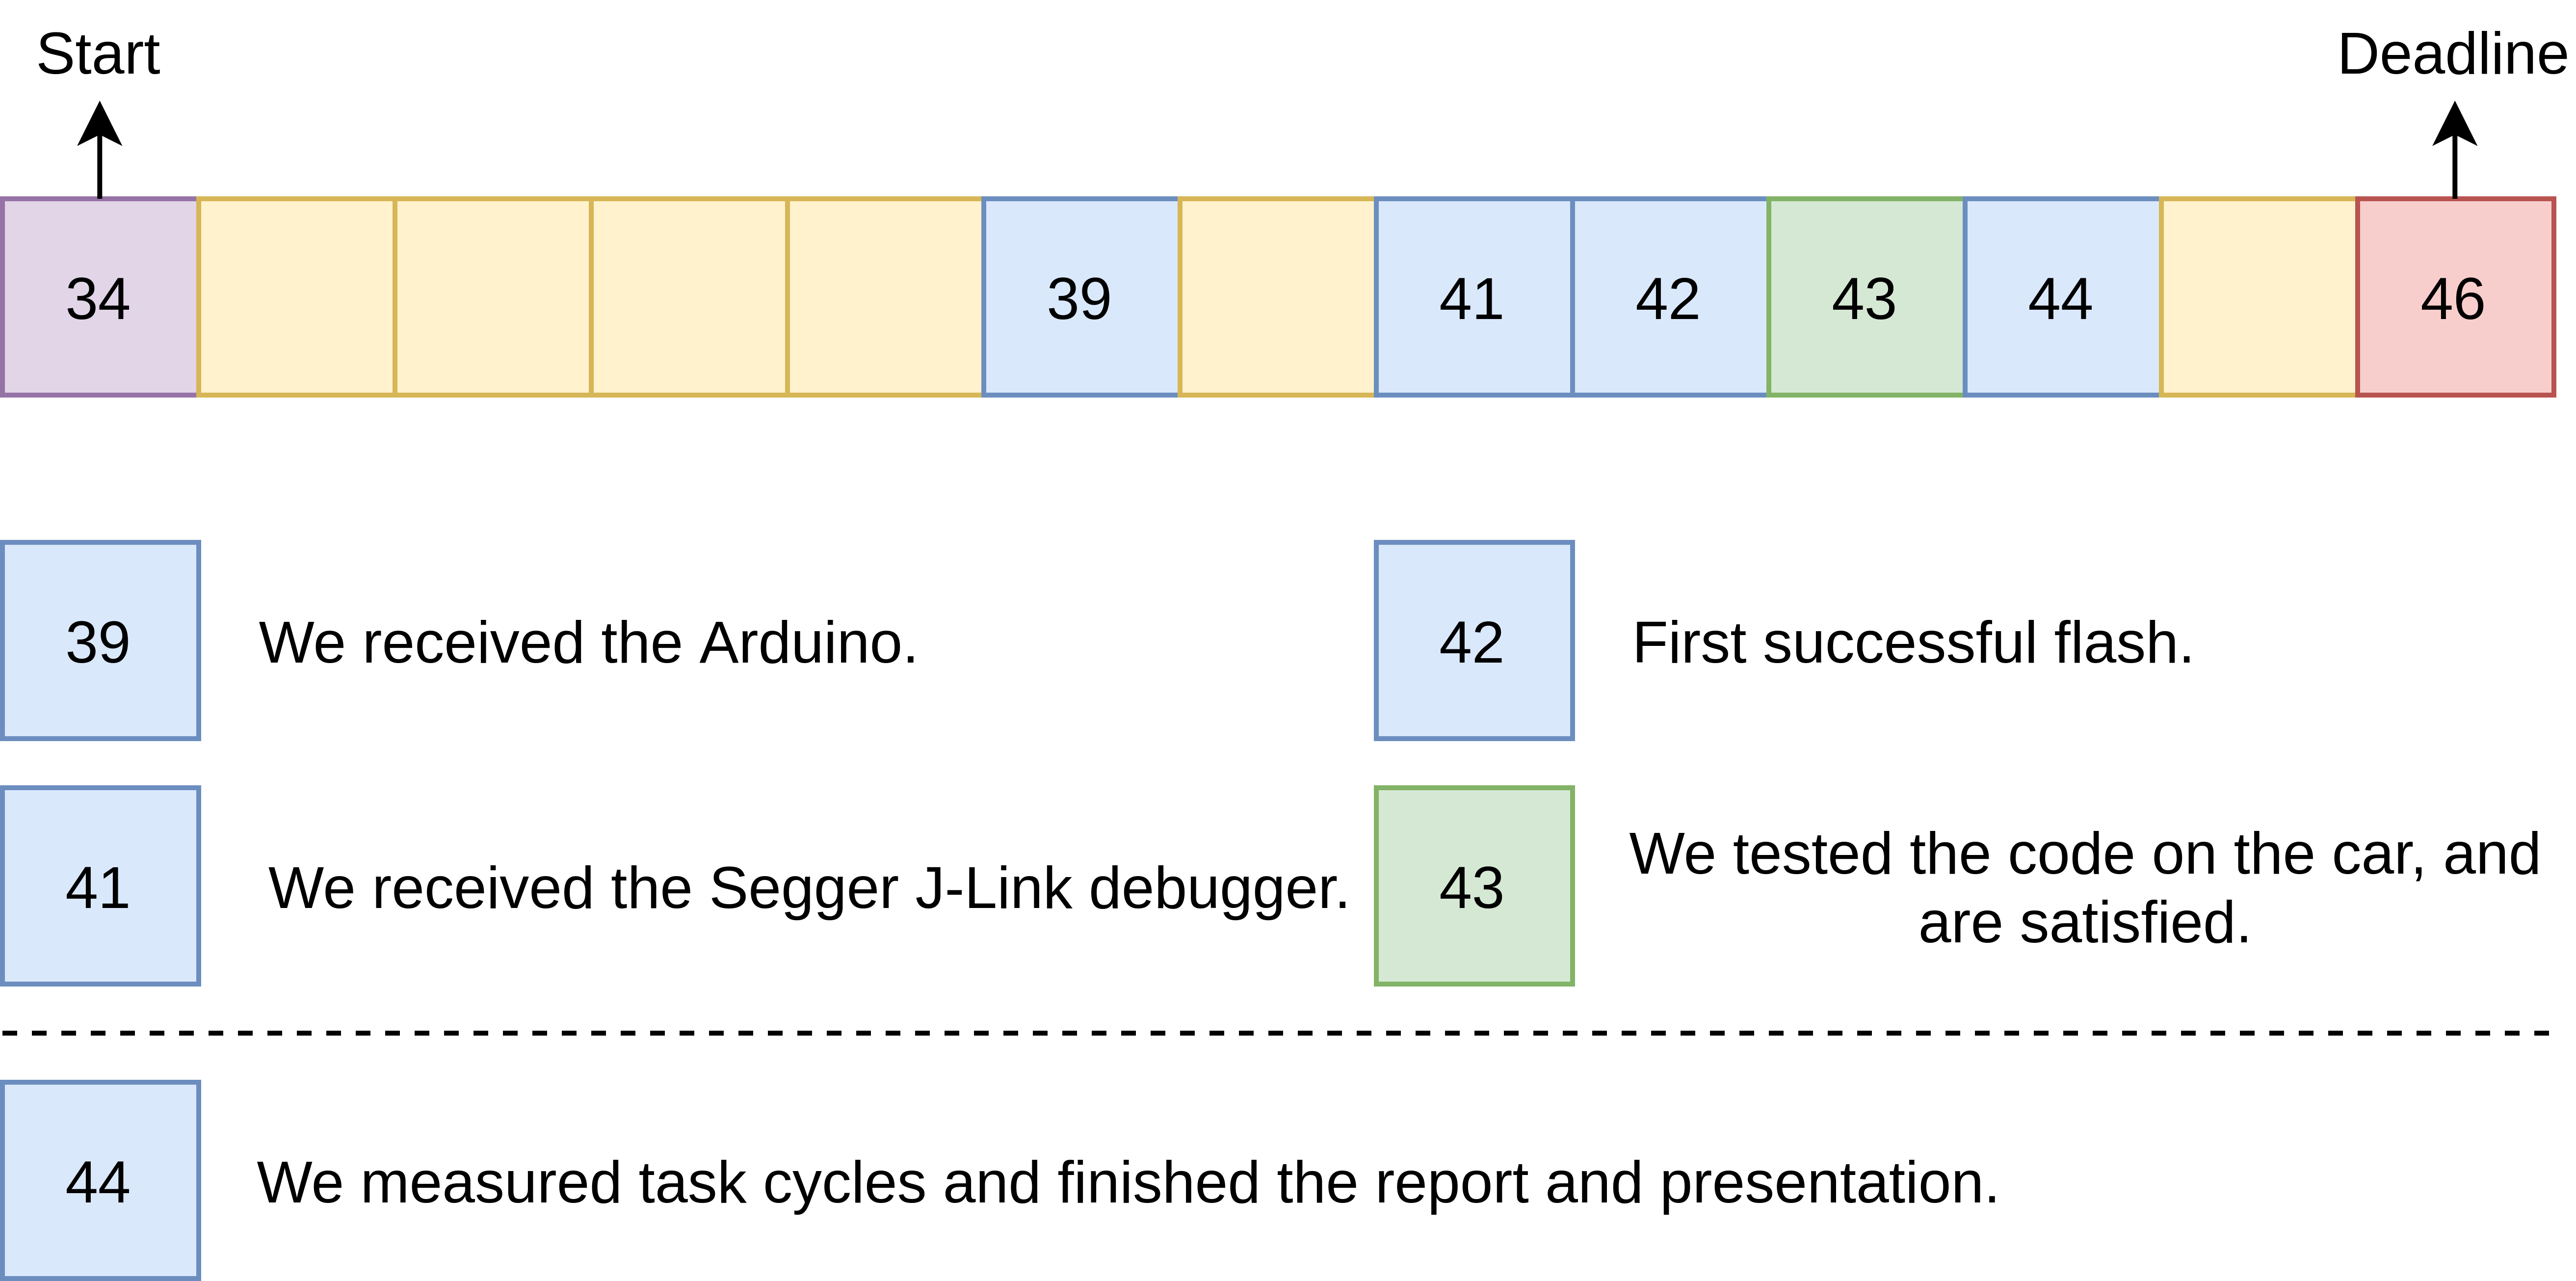
\includegraphics[width=\linewidth]{img/timeline.png}
\end{frame}

\begin{frame}
    \centering
    \frametitle{Initial Concept}
    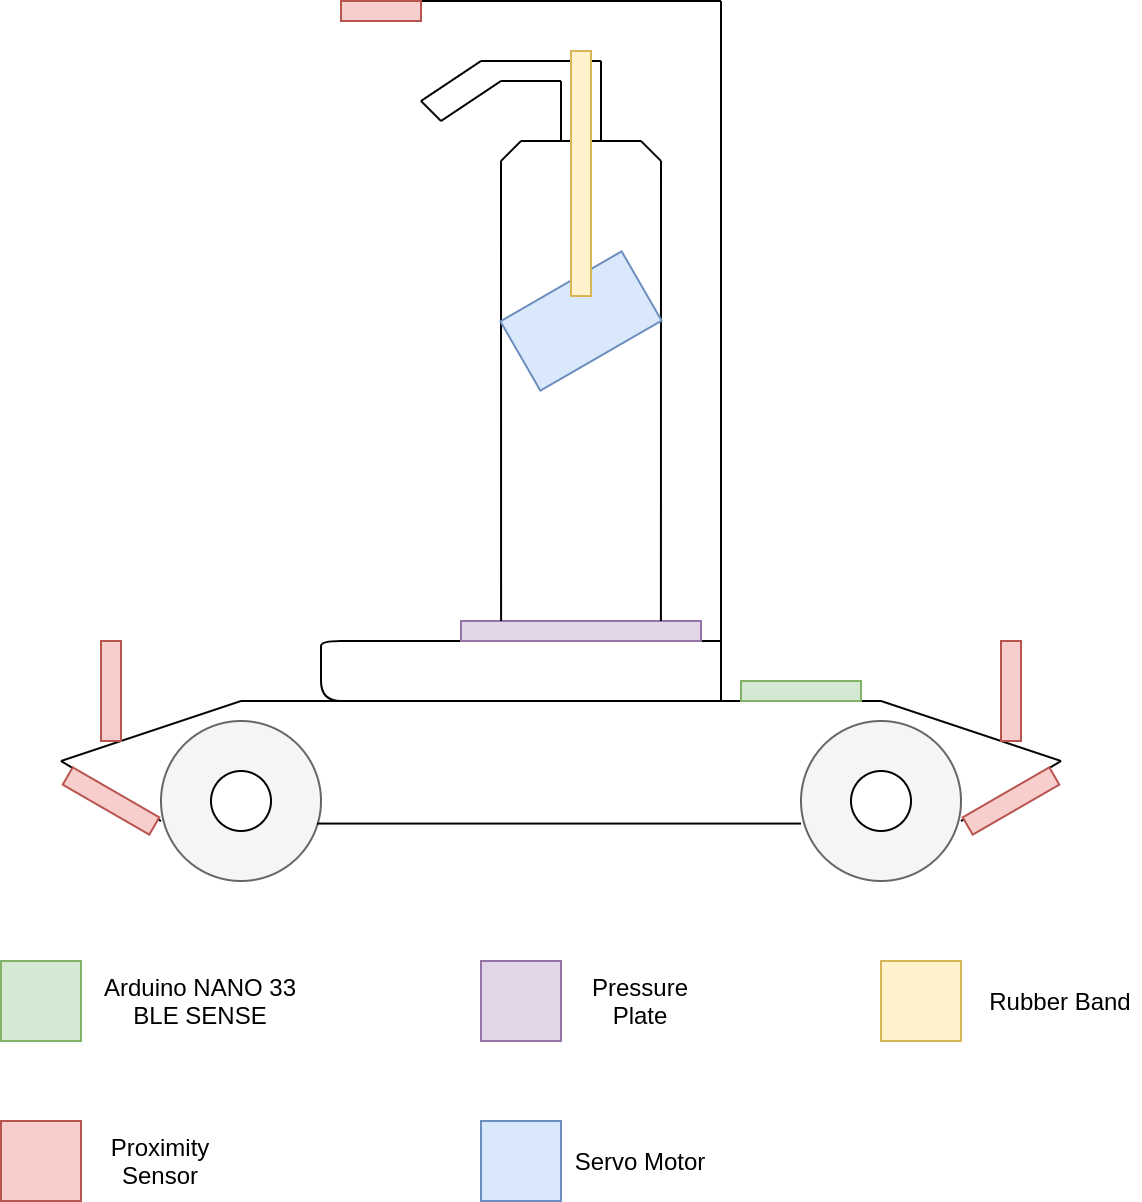
\includegraphics[scale=0.2, keepaspectratio]{img/prototype-drawing.png}
\end{frame}

\begin{frame}
    \frametitle{Final Design}
    \centering
    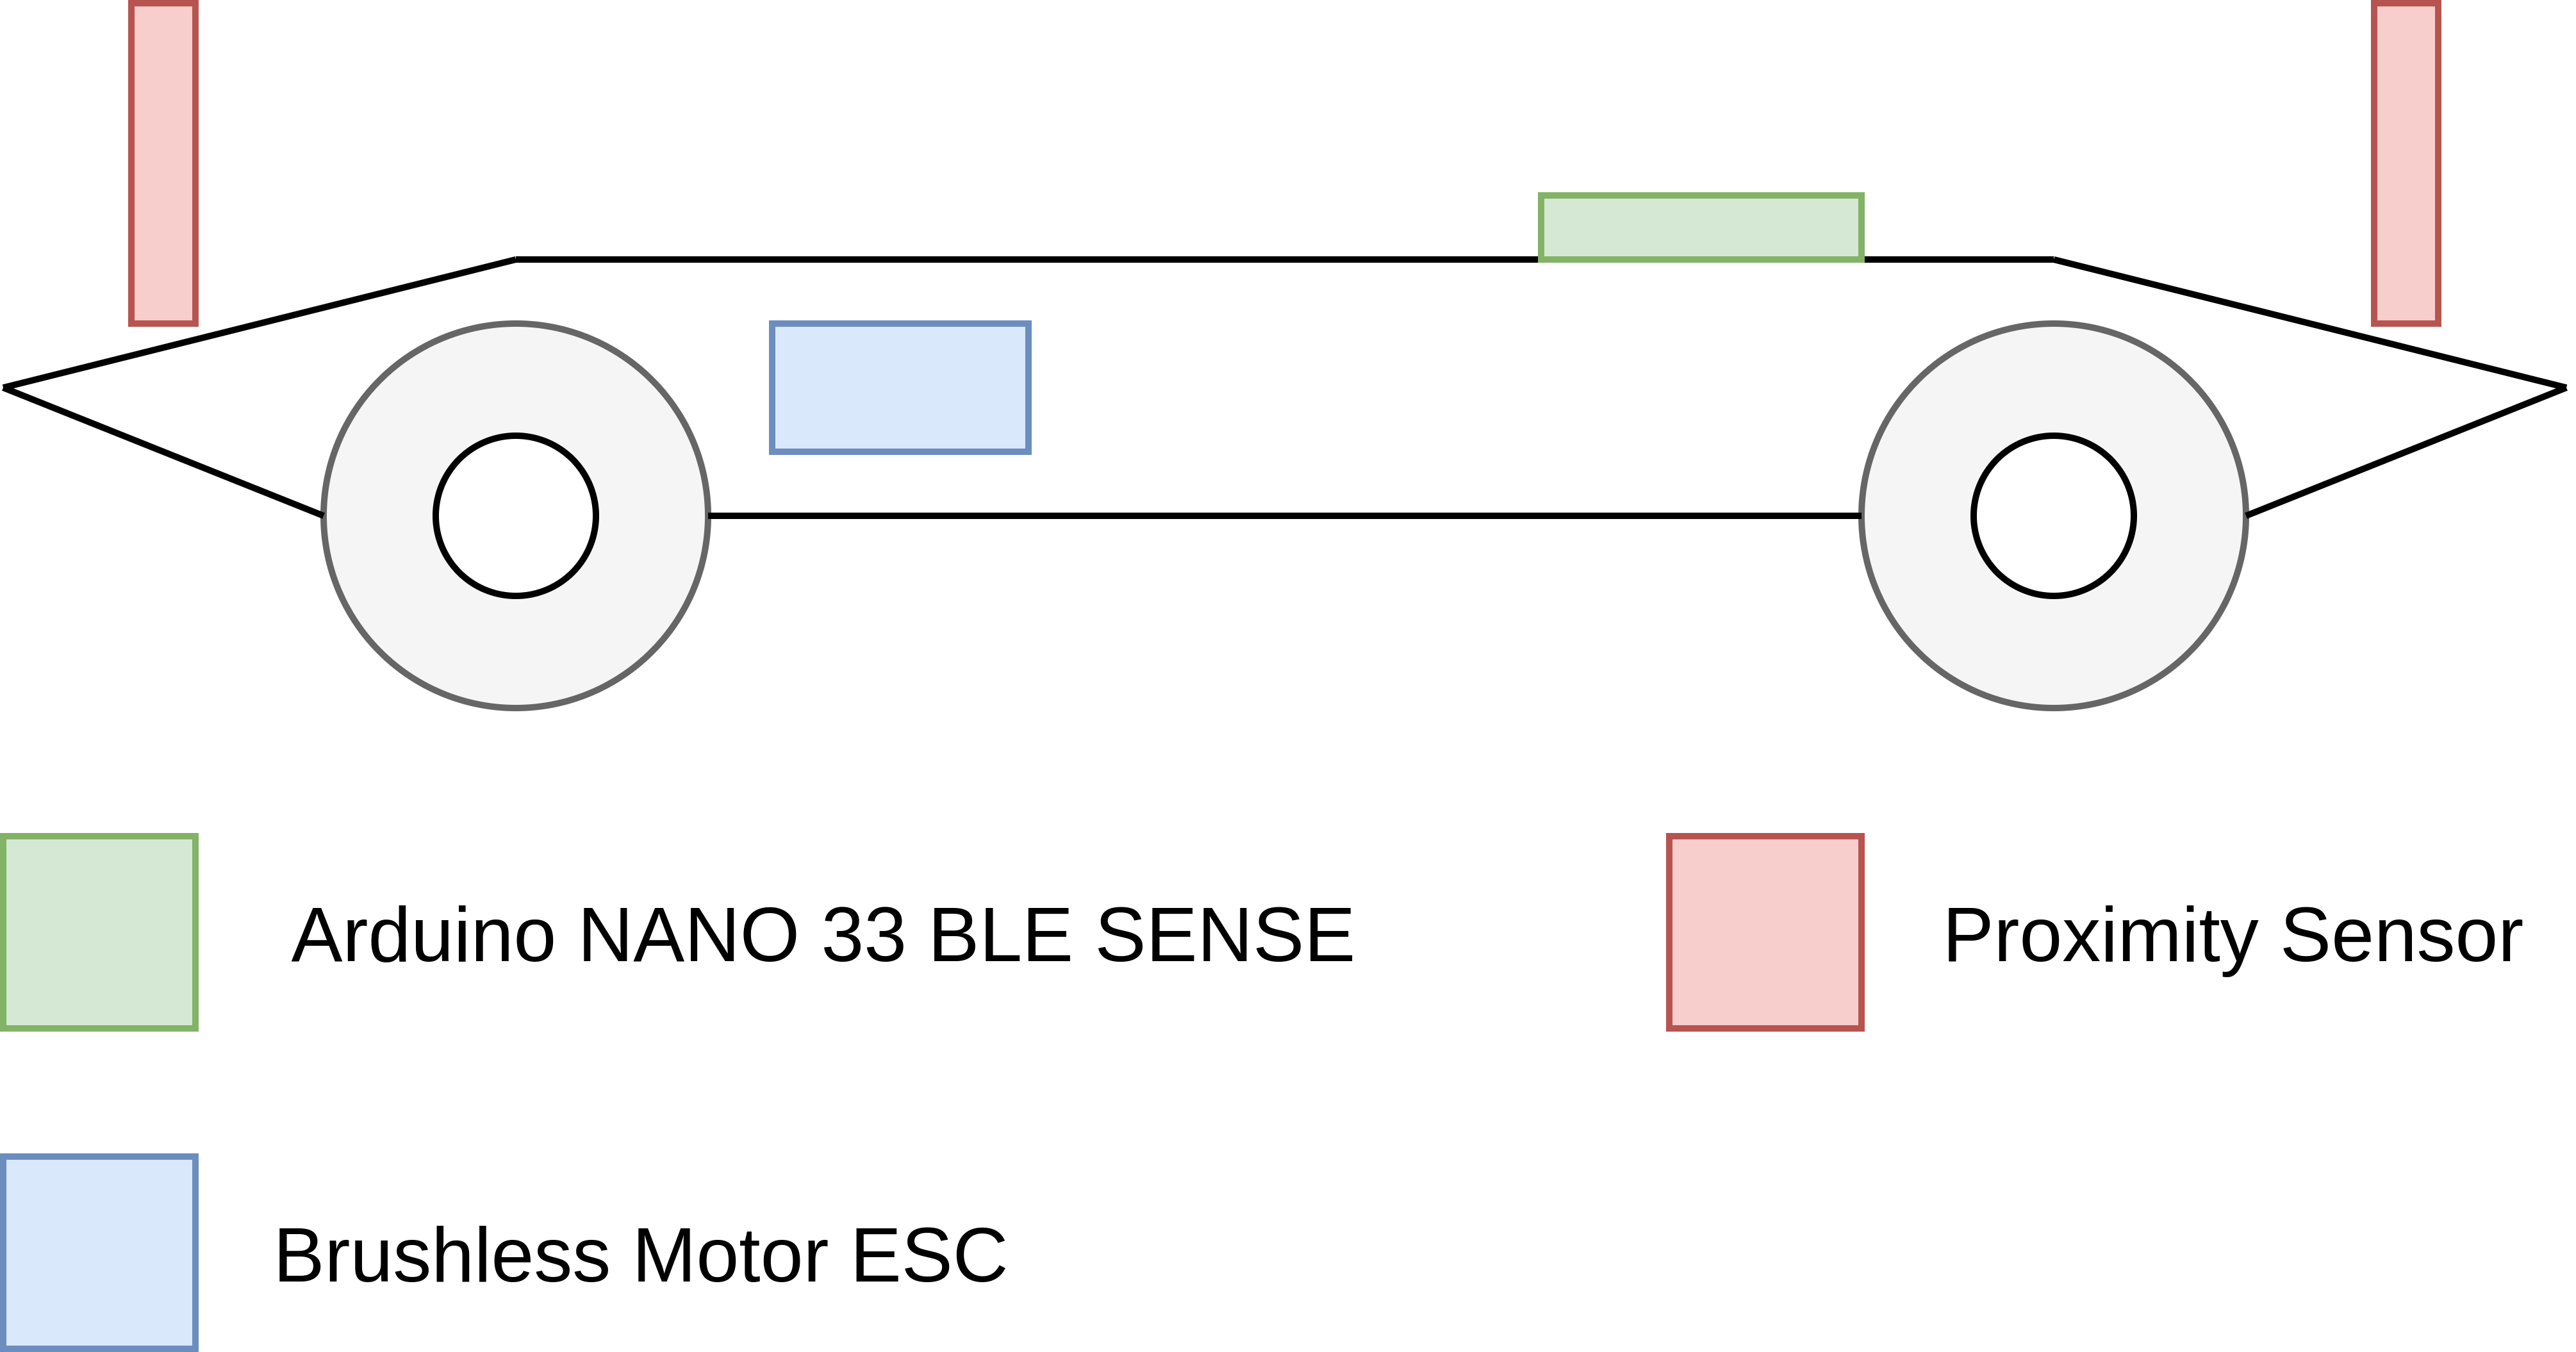
\includegraphics[scale=0.065]{img/final-design.png}
\end{frame}

\begin{frame}
    \frametitle{System Architecture}
    \centering
    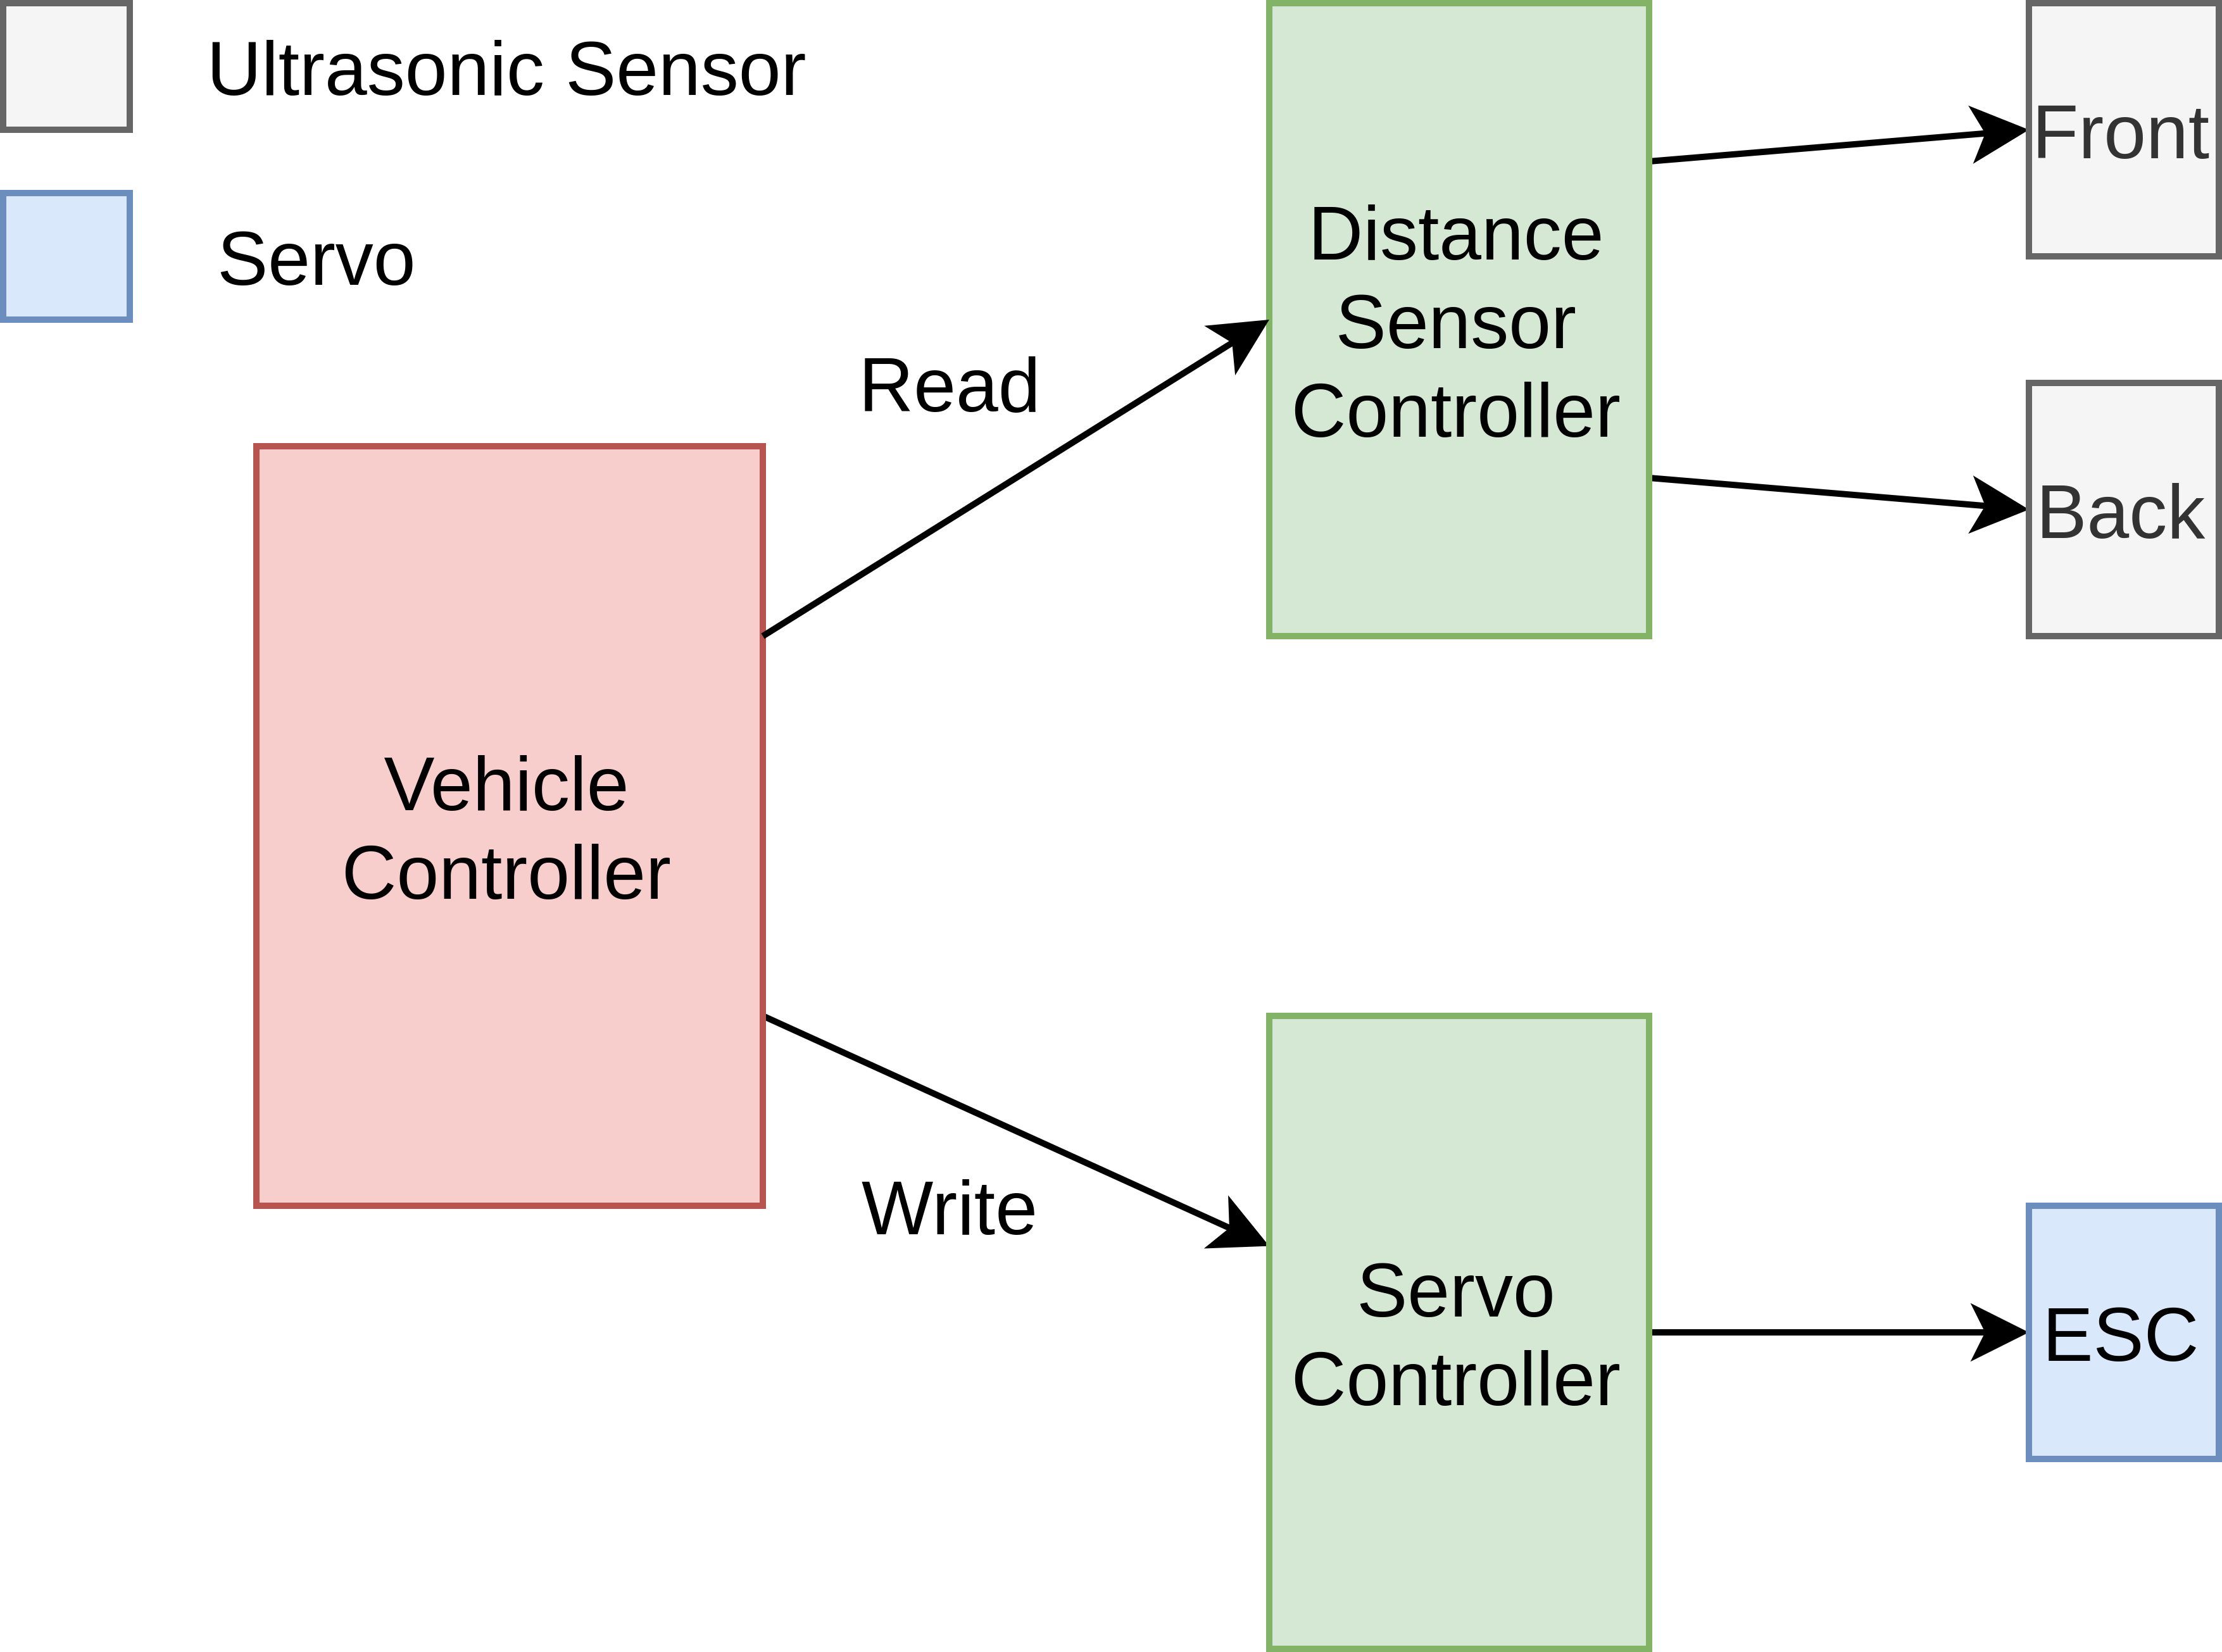
\includegraphics[scale=0.065]{img/system-architecture.png}
\end{frame}

\begin{frame}
    \frametitle{Finite State Machine}
    \centering
    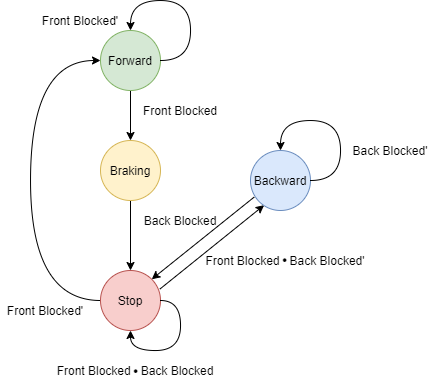
\includegraphics[scale=0.06, keepaspectratio]{img/finite-state-machine.png}
\end{frame}

\begin{frame}
    \frametitle{Distance Sensor}
    \centering
    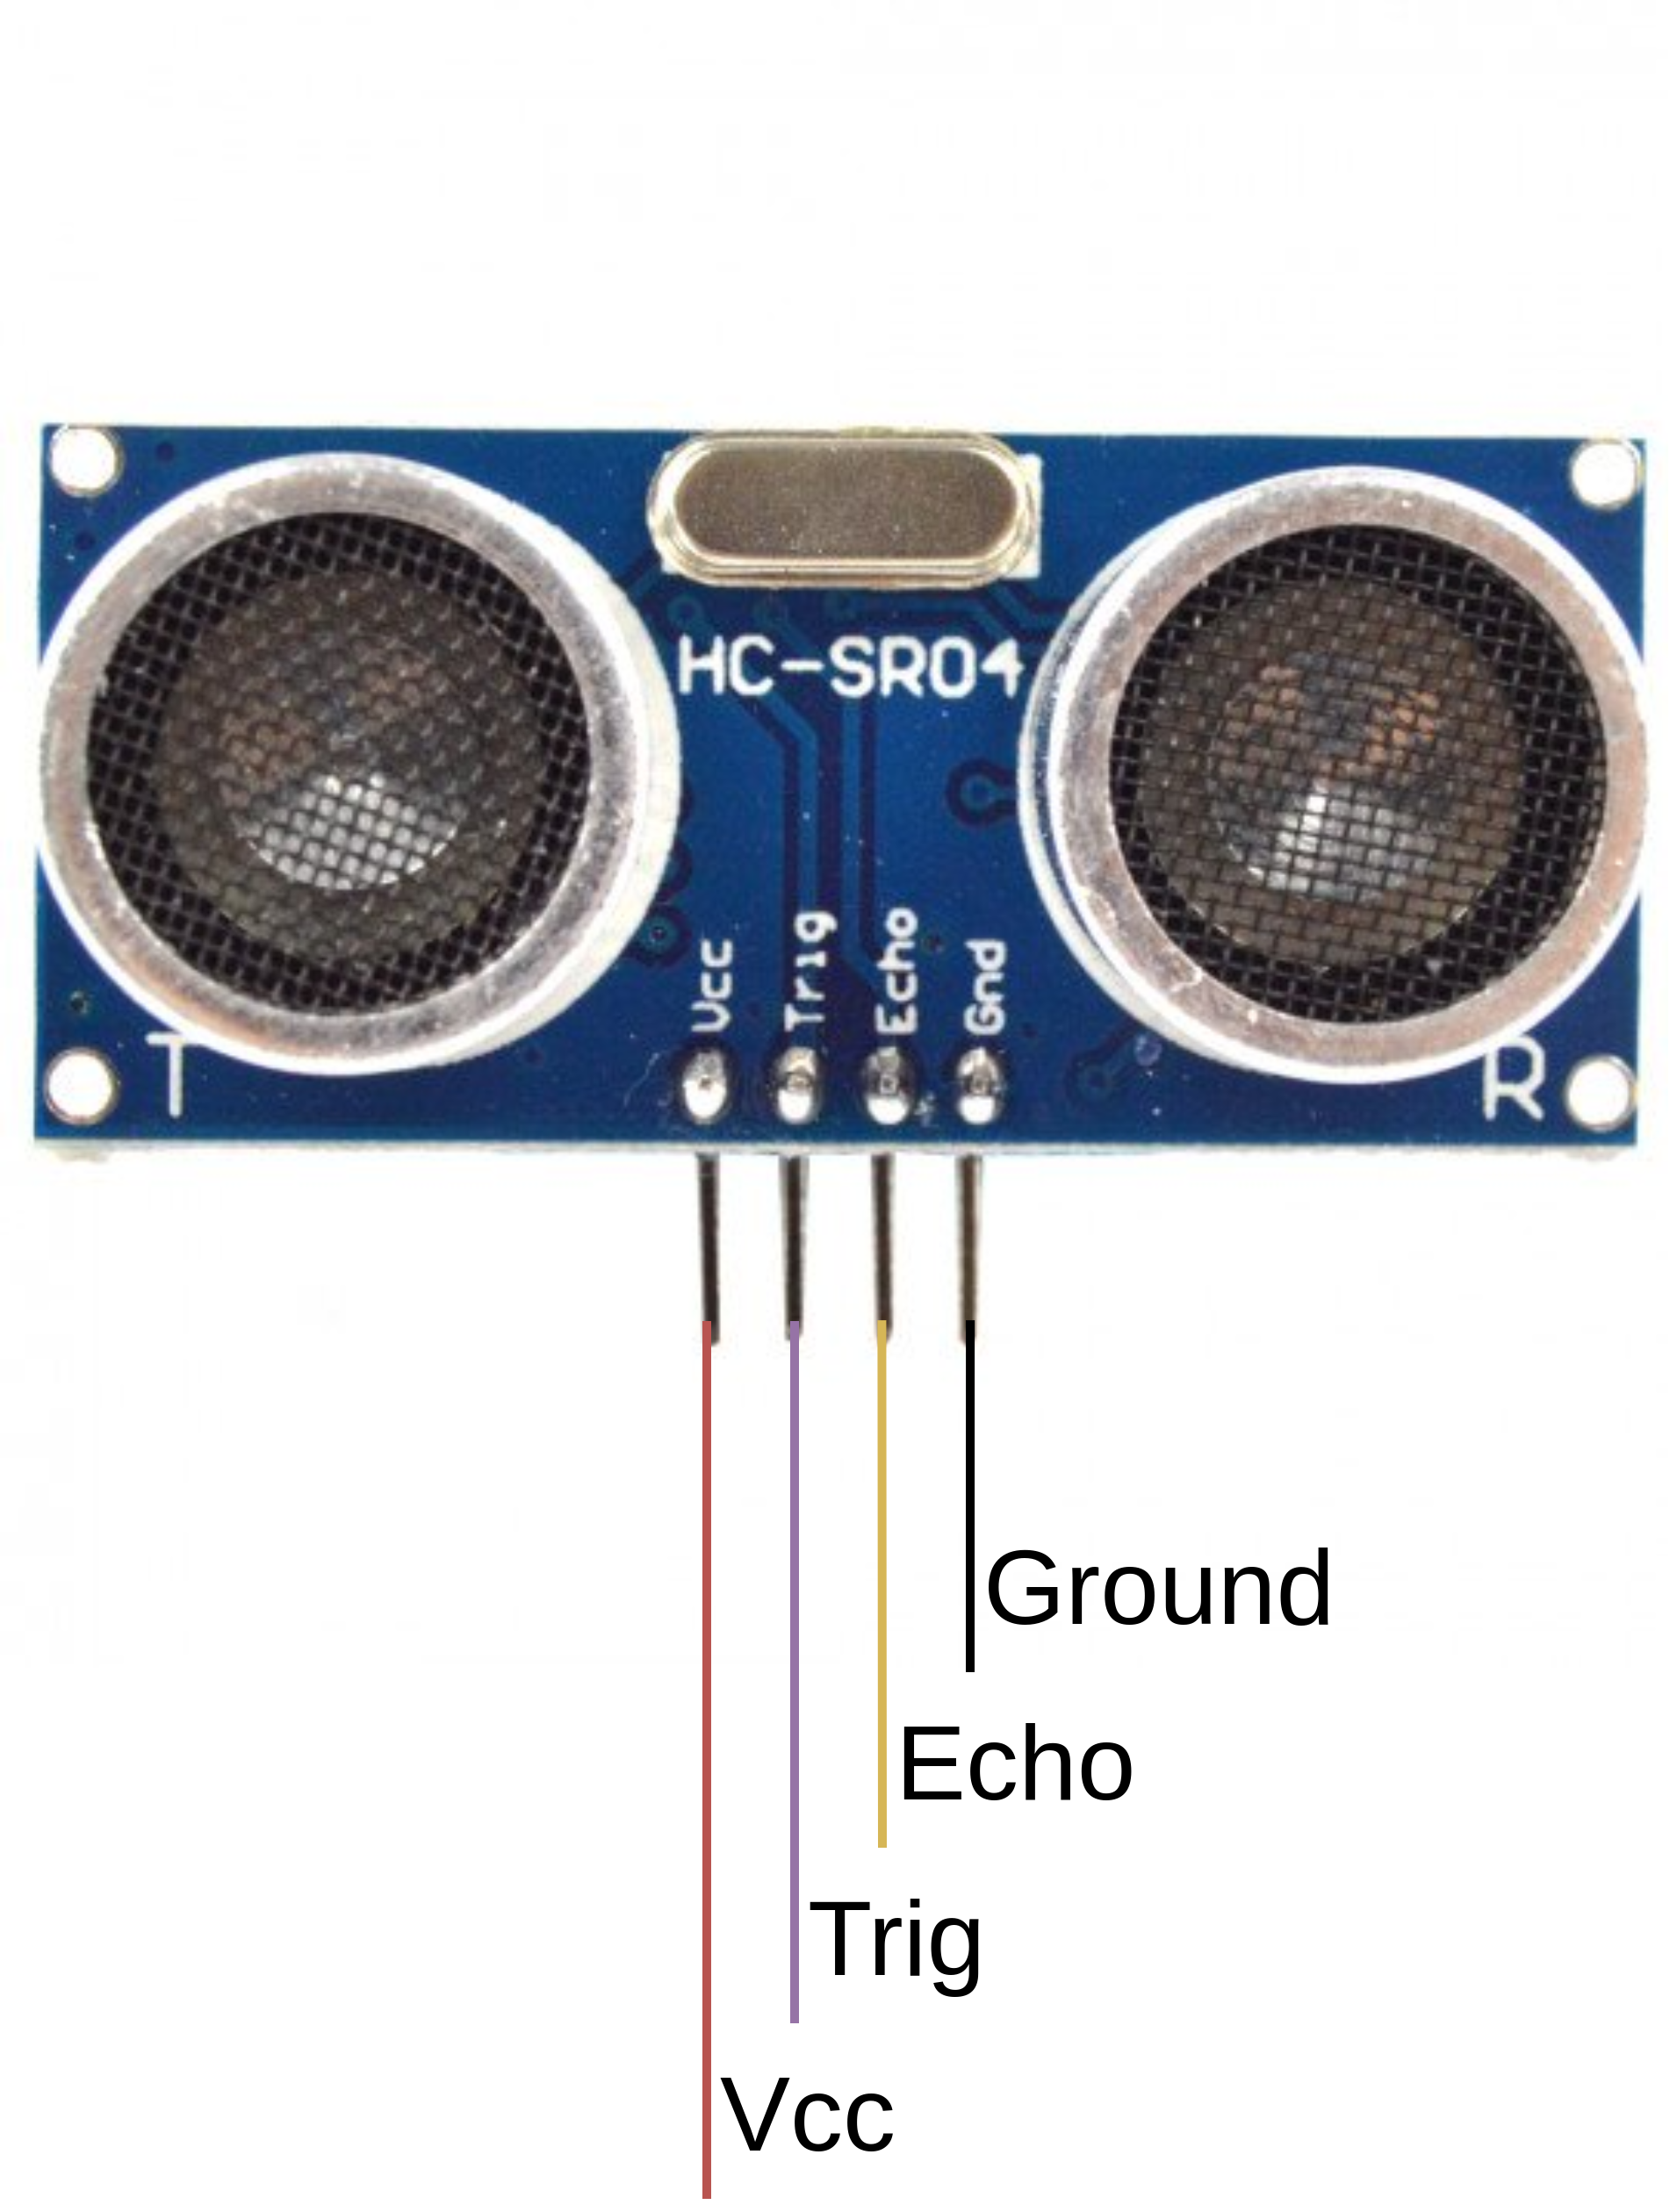
\includegraphics[scale=0.08]{img/hcsr04.png}
\end{frame}

\begin{frame}
    \frametitle{Distance Sensor}
    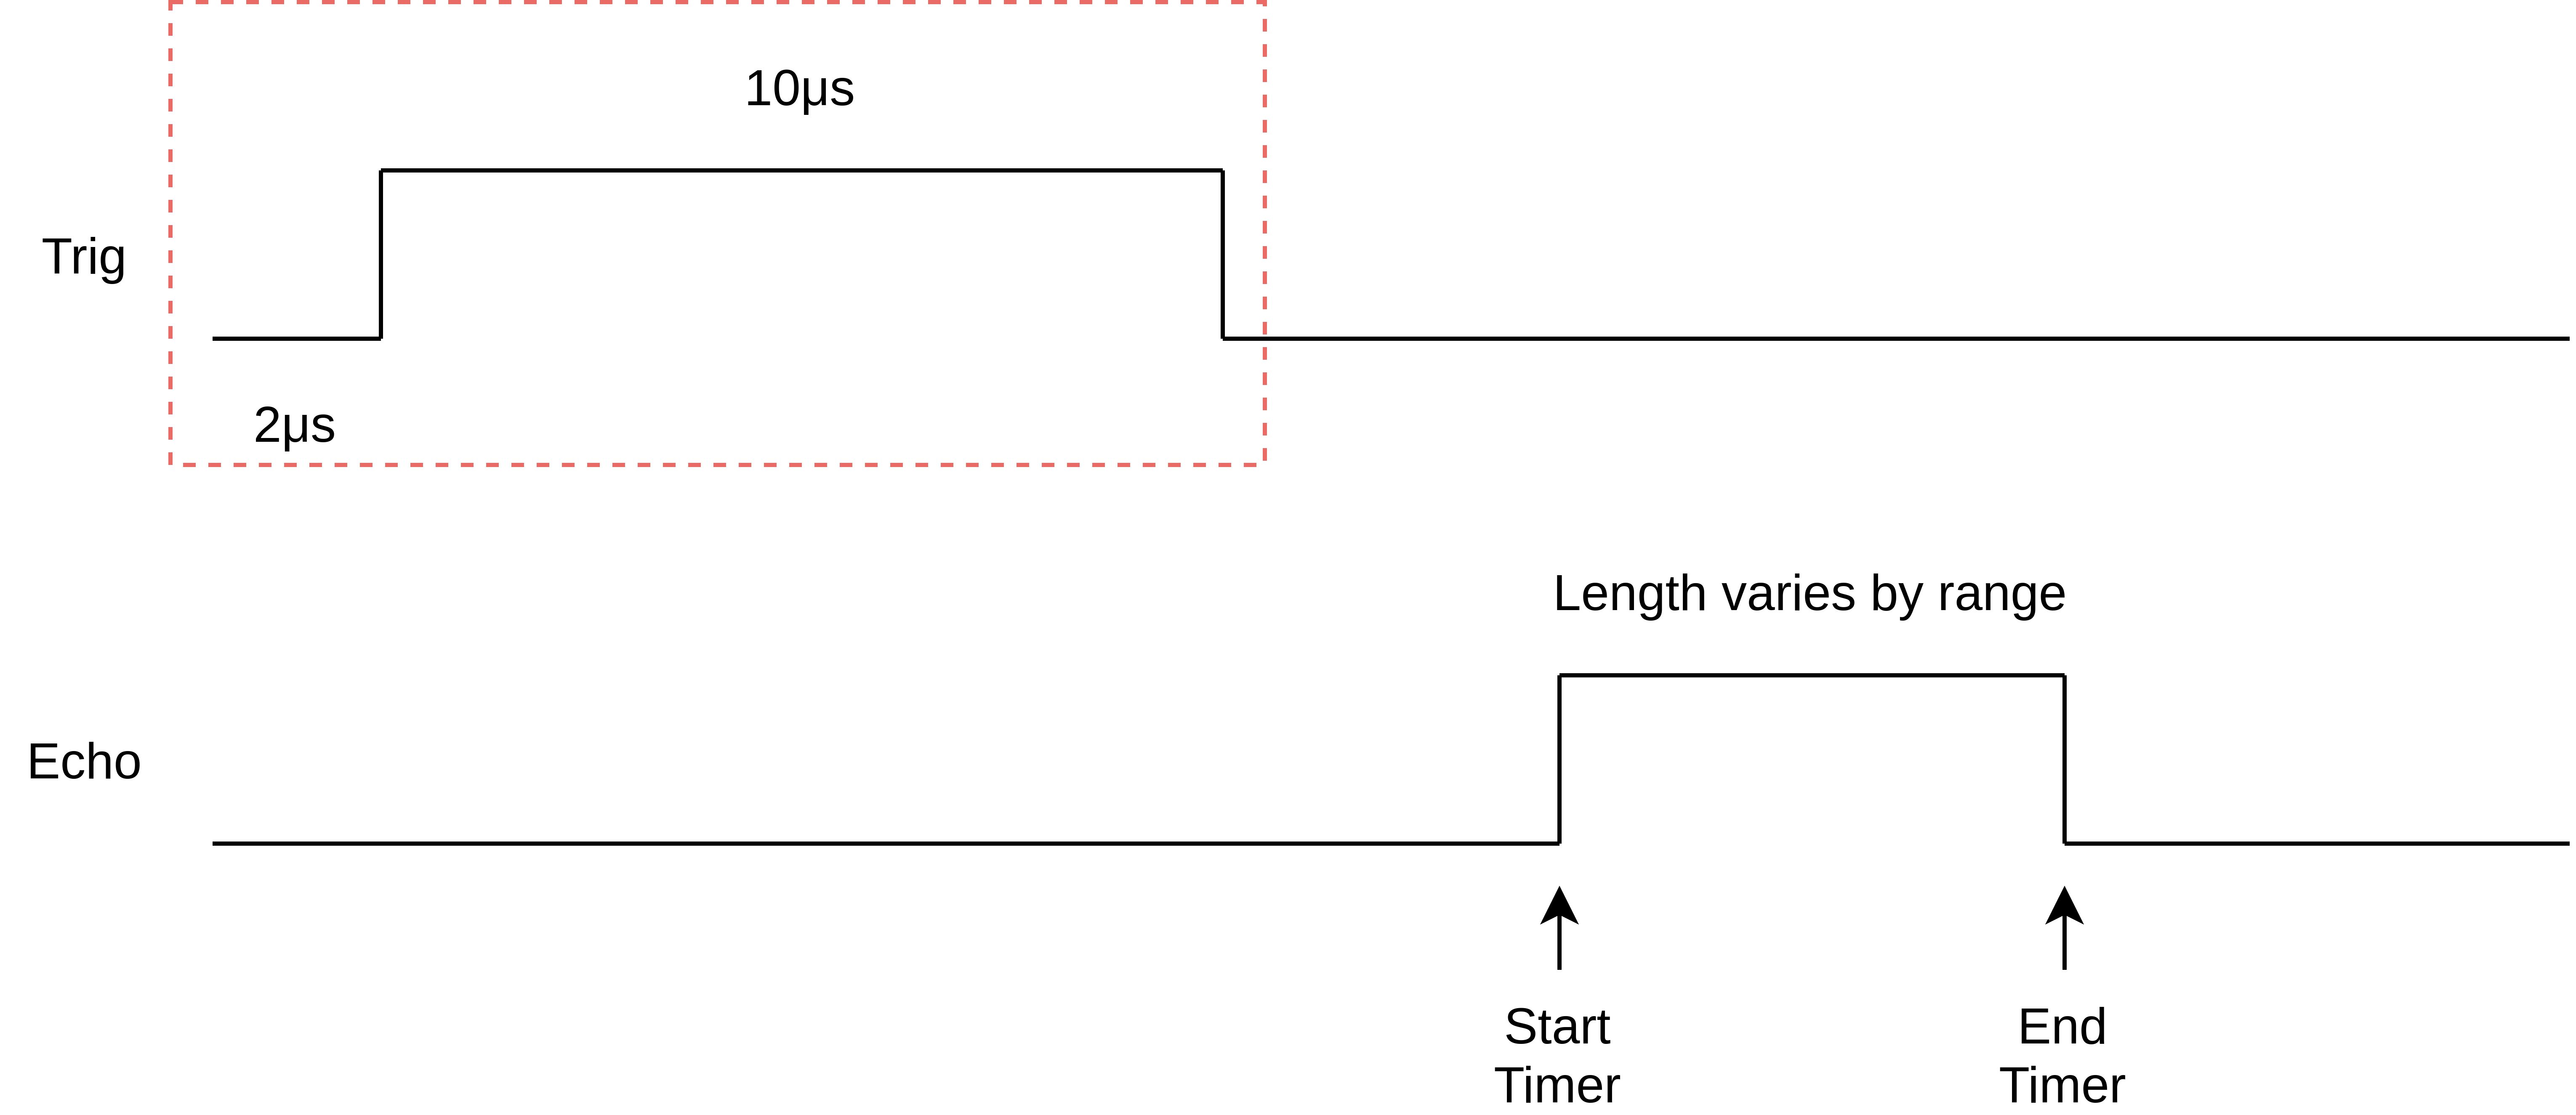
\includegraphics[width=\linewidth]{img/ultrasonic-sensor.png}
\end{frame}

\begin{frame}
    \frametitle{Servo}
    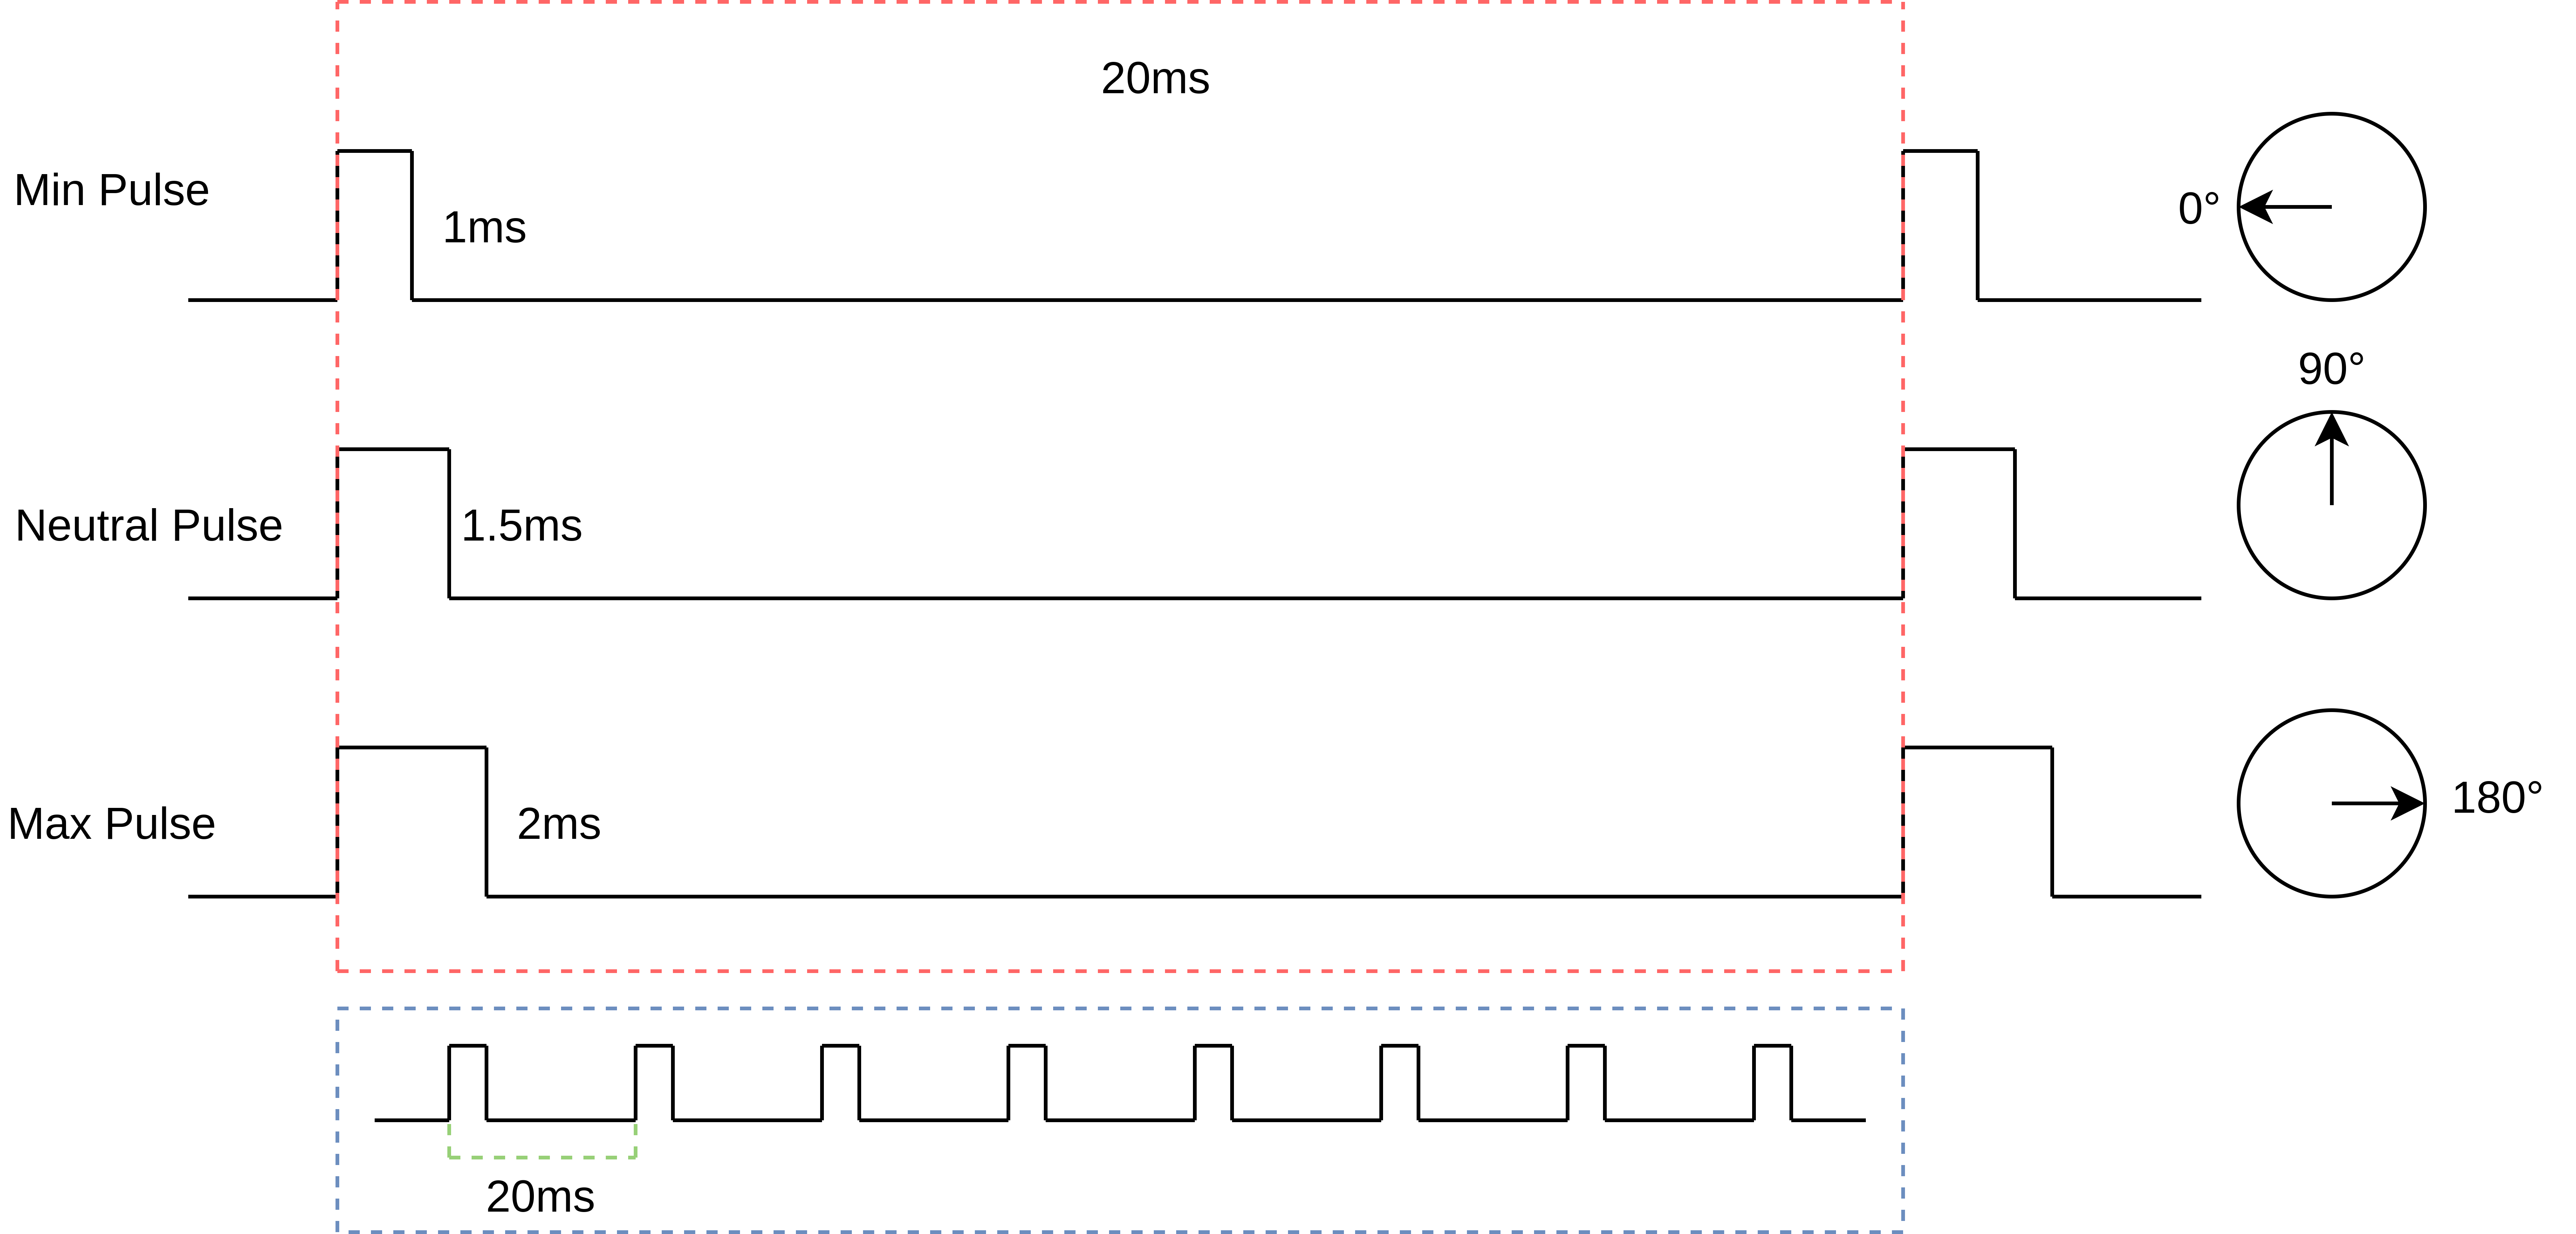
\includegraphics[width=\linewidth]{img/servo.png}
\end{frame}

\begin{frame}
    \frametitle{Brushless Motor ESC}
    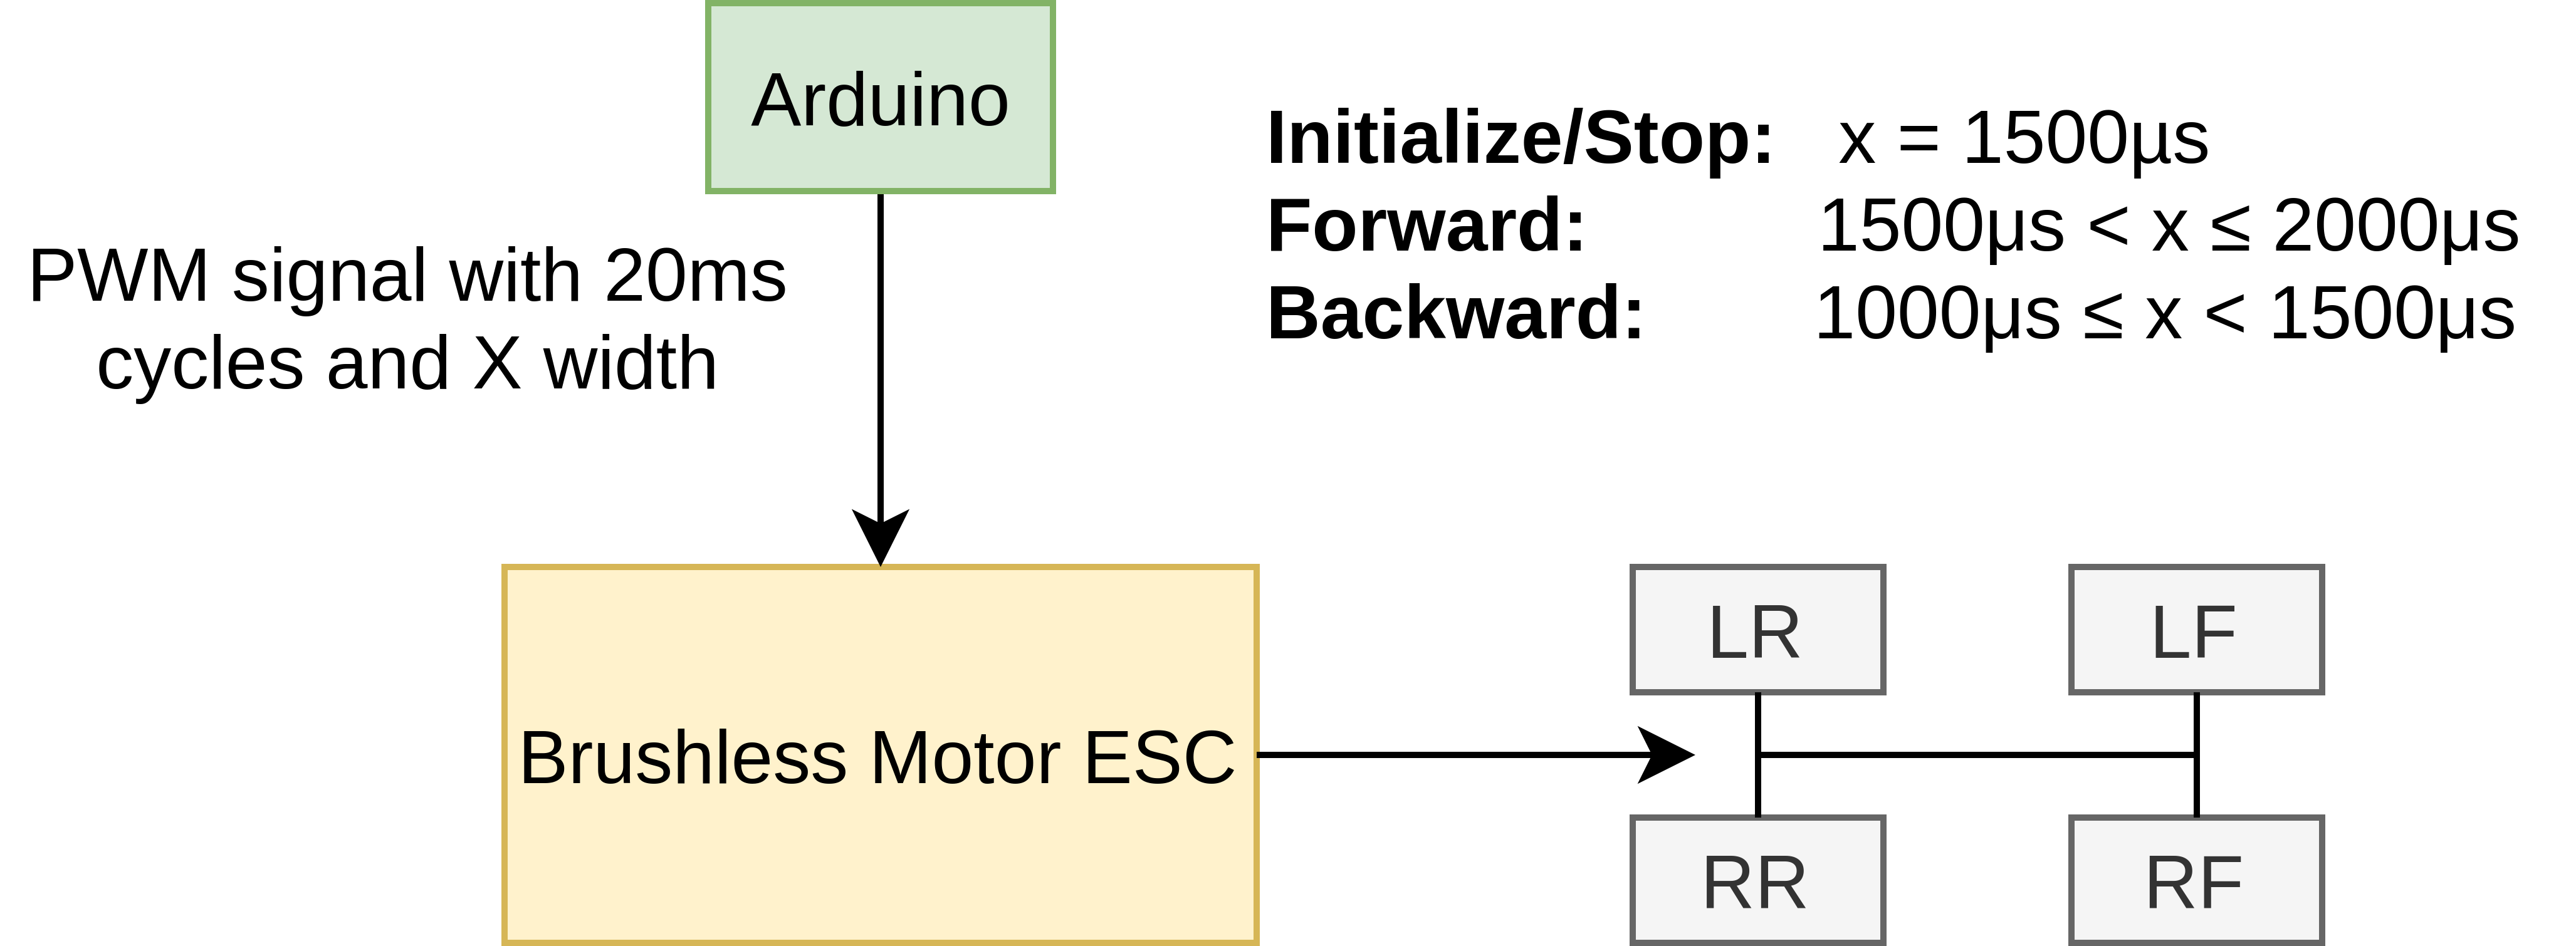
\includegraphics[width=\linewidth]{img/brushless-motor-esc}
\end{frame}

\begin{frame}
    \centering
    \frametitle{Questions}
Any questions?
\end{frame}

\begin{frame}
    \centering
    \frametitle{The End}
    Thank you for your attention. :)\\
    You can find our Ada\_Drivers\_Library fork and the source code over at https://github.com/stykk-gruppen
\end{frame}

\end{document}

padding oracle attacks.
